% Copyright 2004 by Till Tantau <tantau@users.sourceforge.net>.
%
% In principle, this file can be redistributed and/or modified under
% the terms of the GNU Public License, version 2.
%
% However, this file is supposed to be a template to be modified
% for your own needs. For this reason, if you use this file as a
% template and not specifically distribute it as part of a another
% package/program, I grant the extra permission to freely copy and
% modify this file as you see fit and even to delete this copyright
% notice. 

\documentclass{beamer}

% There are many different themes available for Beamer. A comprehensive
% list with examples is given here:
% http://deic.uab.es/~iblanes/beamer_gallery/index_by_theme.html
% You can uncomment the themes below if you would like to use a different
% one:
\usepackage{subcaption}
%\usepackage{hyperref}
%\hypersetup{
%    colorlinks=true,
%    linkcolor=blue,
%    filecolor=magenta,      
%    urlcolor=cyan,
%}
%
%\setbeamertemplate{navigation symbols}{}
%\addtobeamertemplate{navigation symbols}{}{%
%    \usebeamerfont{footline}%
%    \usebeamercolor[fg]{footline}%
%    \hspace{1em}%
%    \insertframenumber/\inserttotalframenumber
%}
%\usetheme{AnnArbor}
%\usetheme{Antibes}
%\usetheme{Bergen}
%\usetheme{Berkeley}
%\usetheme{Berlin}
%\usetheme{Boadilla}
%\usetheme{boxes}
%\usetheme{CambridgeUS}
%\usetheme{Copenhagen}
%\usetheme{Darmstadt}
\usetheme{default}
%\usetheme{Frankfurt}
%\usetheme{Goettingen}
%\usetheme{Hannover}
%\usetheme{Ilmenau}
%\usetheme{JuanLesPins}
%\usetheme{Luebeck}
%\usetheme{Madrid}
%\usetheme{Malmoe}
%\usetheme{Marburg}
%\usetheme{Montpellier}
%\usetheme{PaloAlto}
%\usetheme{Pittsburgh}
%\usetheme{Rochester}
%\usetheme{Singapore}
%\usetheme{Szeged}
%\usetheme{Warsaw}
% Let's get started
\begin{document}

%\begin{frame}
 % \titlepage
%end{frame}

%\begin{frame}{Outline}
%  \tableofcontents
  % You might wish to add the option [pausesections]
%\end{frame}

% Section and subsections will appear in the presentation overview
% and table of contents.
%\section{First Main Section}

%\subsection{First Subsection}

\begin{frame}
  \begin{figure}[!h]
  \captionsetup[subfigure]{labelformat=empty}
  \begin{subfigure}{.5\textwidth}
  \centering
  \includegraphics[width=5cm]{reconstructed_top_mass_tw.eps}
  \caption{Chongbin(python)}
  \end{subfigure} \hfill
  \begin{subfigure}{.5\textwidth}
  \centering
  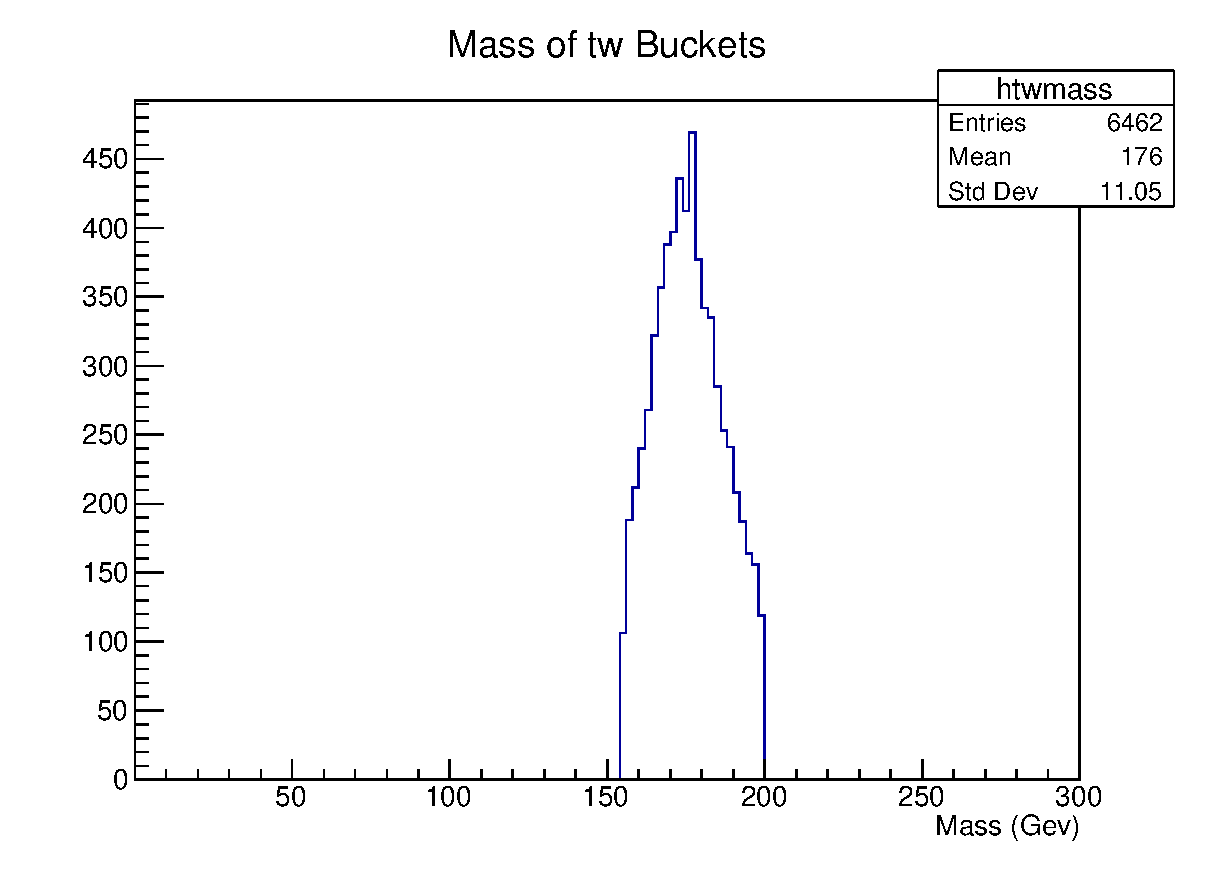
\includegraphics[width=5cm]{htwmass_alljetregion.eps}
  \caption{TTHbb}
  \end{subfigure}
  \end{figure}
\end{frame}

\begin{frame}
  \begin{figure}[!h]
  \captionsetup[subfigure]{labelformat=empty}
  \begin{subfigure}{.5\textwidth}
  \centering
  \includegraphics[width=5cm]{reconstructed_top_pt_tw.eps}
  \caption{Chongbin(python)}
  \end{subfigure} \hfill
  \begin{subfigure}{.5\textwidth}
  \centering
  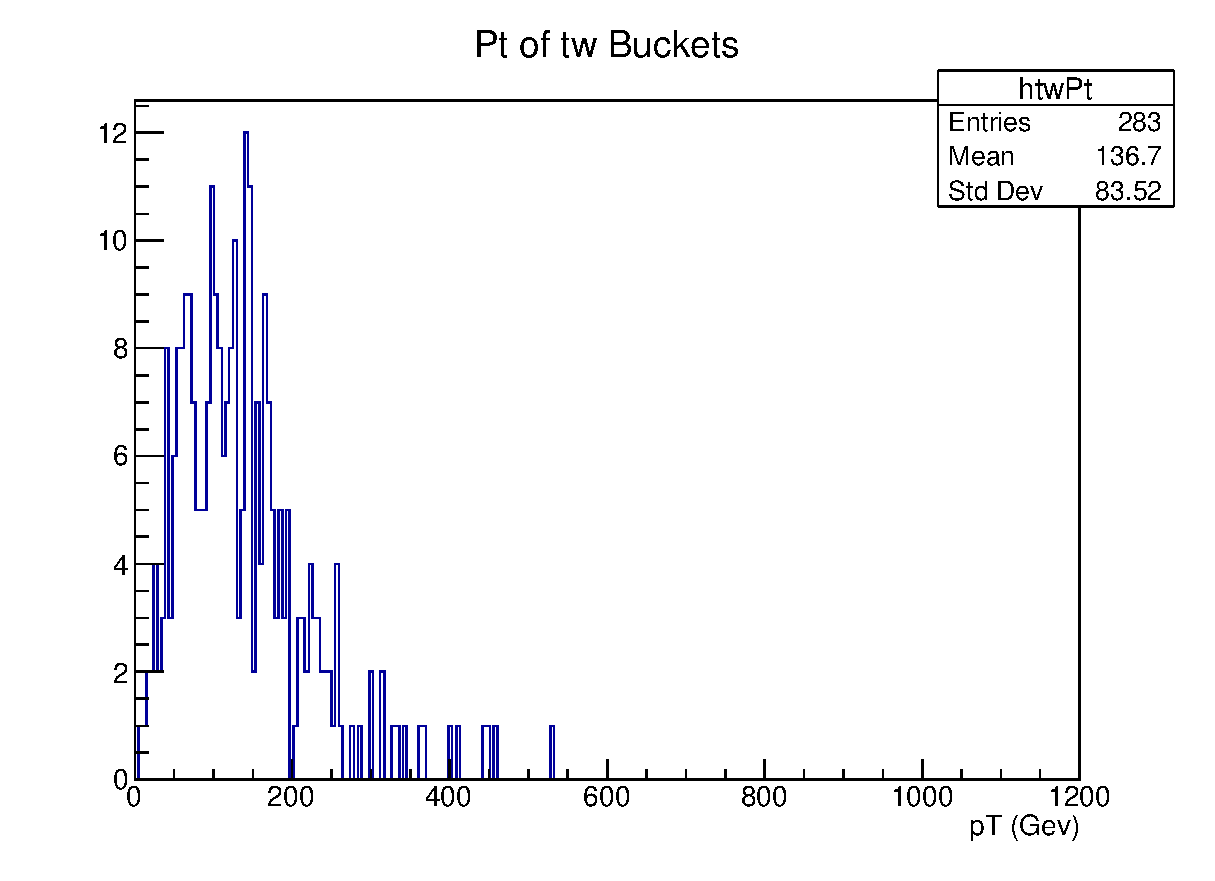
\includegraphics[width=5cm]{htwPt_alljetregion.eps}
  \caption{TTHbb}
  \end{subfigure}
  \end{figure}
\end{frame}

\begin{frame}
  \begin{figure}[!h]
  \captionsetup[subfigure]{labelformat=empty}
  \begin{subfigure}{.5\textwidth}
  \centering
  \includegraphics[width=5cm]{reconstructed_top_eta_tw.eps}
  \caption{Chongbin(python)}
  \end{subfigure} \hfill
  \begin{subfigure}{.5\textwidth}
  \centering
  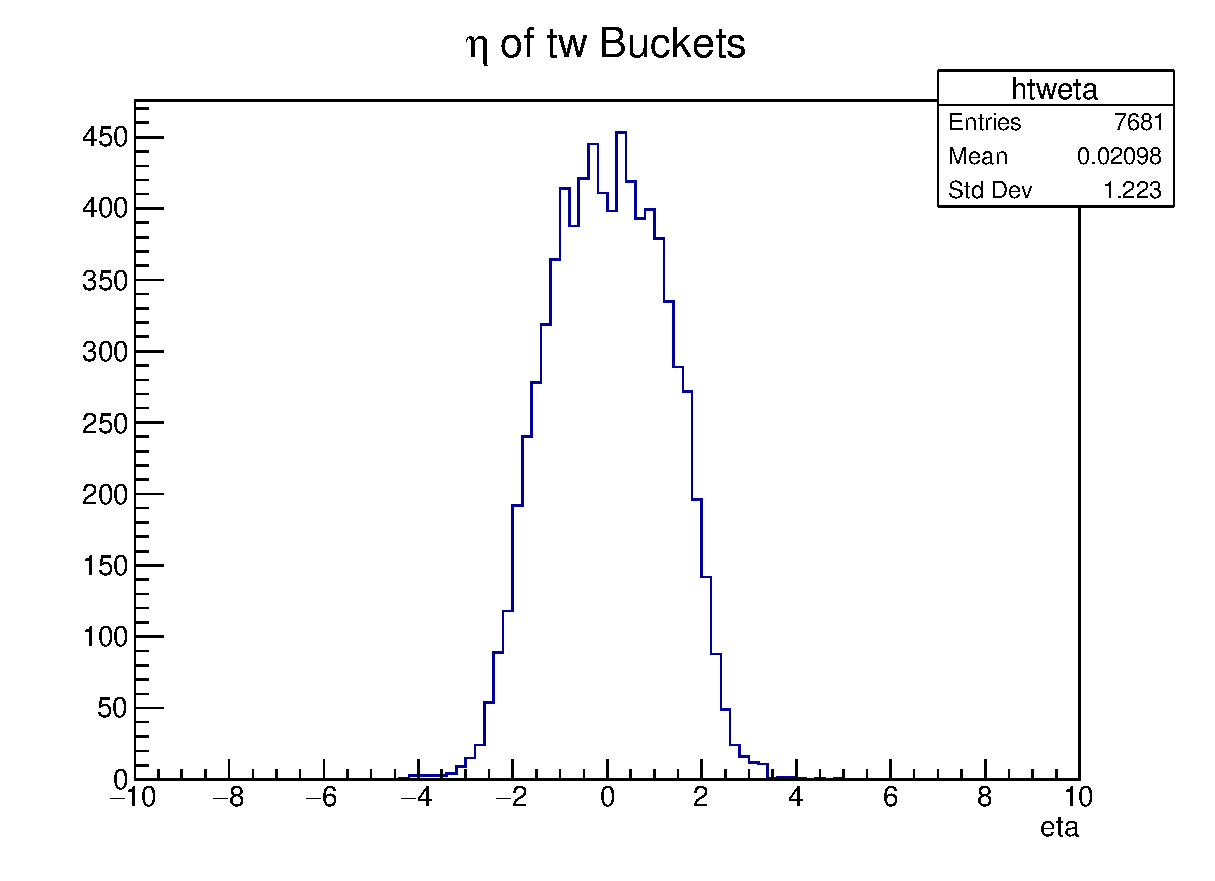
\includegraphics[width=5cm]{htweta_alljetregion.eps}
  \caption{TTHbb}
  \end{subfigure}
  \end{figure}
\end{frame}

\begin{frame}
  \begin{figure}[!h]
  \captionsetup[subfigure]{labelformat=empty}
  \begin{subfigure}{.5\textwidth}
  \centering
  \includegraphics[width=5cm]{reconstructed_top_mass_t_.eps}
  \caption{Chongbin(python)}
  \end{subfigure} \hfill
  \begin{subfigure}{.5\textwidth}
  \centering
  \includegraphics[width=5cm]{htminmass_alljetregion.eps}
  \caption{TTHbb}
  \end{subfigure}
  \end{figure}
\end{frame}

\begin{frame}
  \begin{figure}[!h]
  \captionsetup[subfigure]{labelformat=empty}
  \begin{subfigure}{.5\textwidth}
  \centering
  \includegraphics[width=5cm]{reconstructed_top_pt_t_.eps}
  \caption{Chongbin(python)}
  \end{subfigure} \hfill
  \begin{subfigure}{.5\textwidth}
  \centering
  \includegraphics[width=5cm]{htminPt_alljetregion.eps}
  \caption{TTHbb}
  \end{subfigure}
  \end{figure}
\end{frame}

\begin{frame}
  \begin{figure}[!h]
  \captionsetup[subfigure]{labelformat=empty}
  \begin{subfigure}{.5\textwidth}
  \centering
  \includegraphics[width=5cm]{reconstructed_top_eta_t_.eps}
  \caption{Chongbin(python)}
  \end{subfigure} \hfill
  \begin{subfigure}{.5\textwidth}
  \centering
  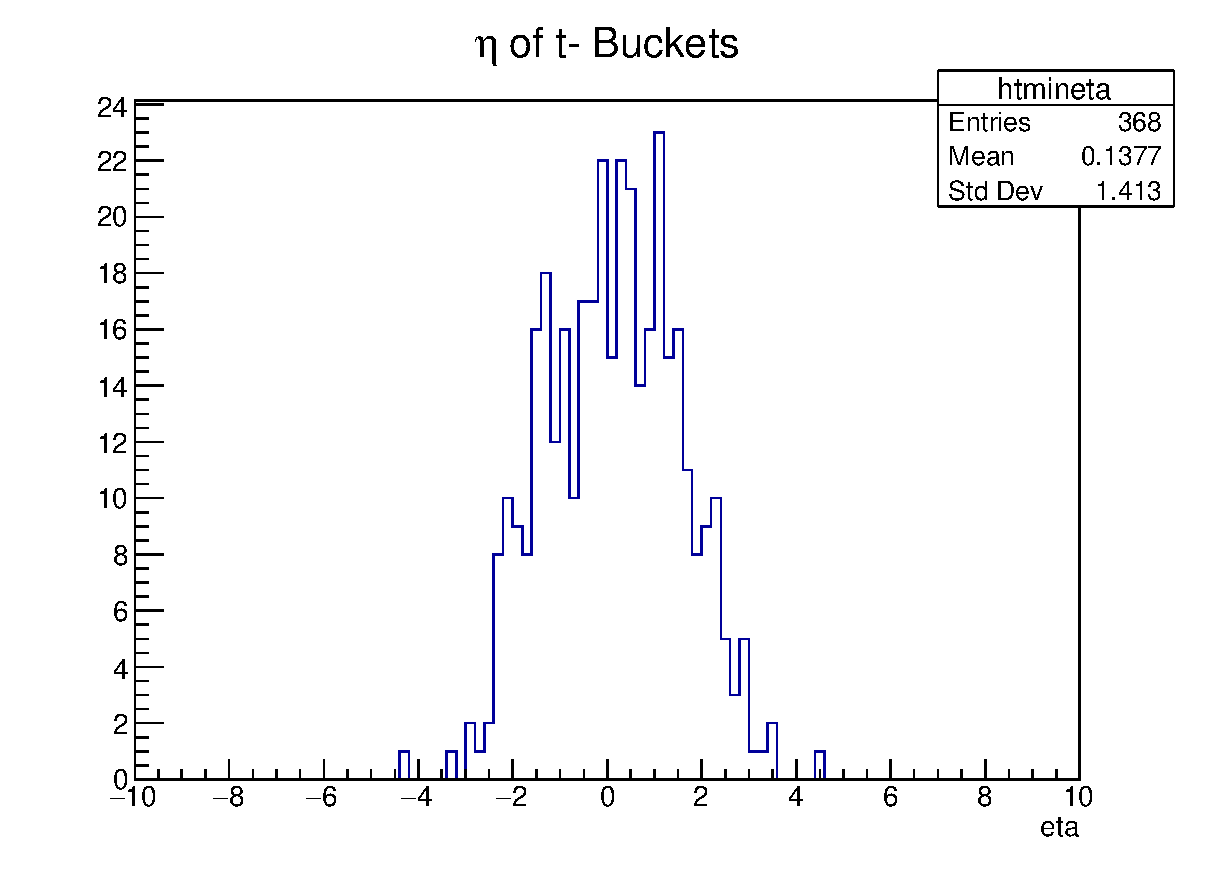
\includegraphics[width=5cm]{htmineta_alljetregion.eps}
  \caption{TTHbb}
  \end{subfigure}
  \end{figure}
\end{frame}

\begin{frame}
  \begin{figure}[!h]
  \captionsetup[subfigure]{labelformat=empty}
  \begin{subfigure}{.5\textwidth}
  \centering
  \includegraphics[width=5cm]{reconstructed_top_mass_t0.eps}
  \caption{Chongbin(python)}
  \end{subfigure} \hfill
  \begin{subfigure}{.5\textwidth}
  \centering
  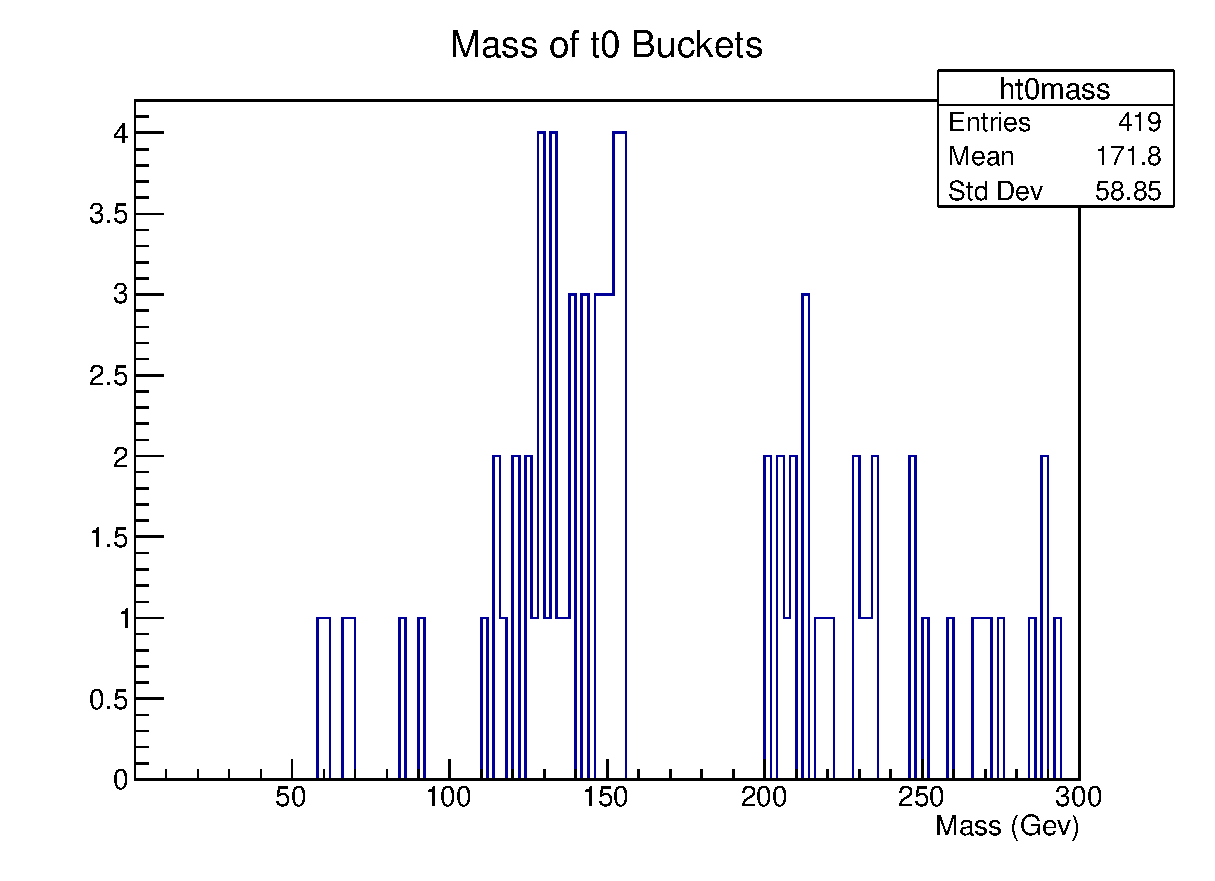
\includegraphics[width=5cm]{ht0mass_alljetregion.eps}
  \caption{TTHbb}
  \end{subfigure}
  \end{figure}
\end{frame}

\begin{frame}
  \begin{figure}[!h]
  \captionsetup[subfigure]{labelformat=empty}
  \begin{subfigure}{.5\textwidth}
  \centering
  \includegraphics[width=5cm]{reconstructed_top_pt_t0.eps}
  \caption{Chongbin(python)}
  \end{subfigure} \hfill
  \begin{subfigure}{.5\textwidth}
  \centering
  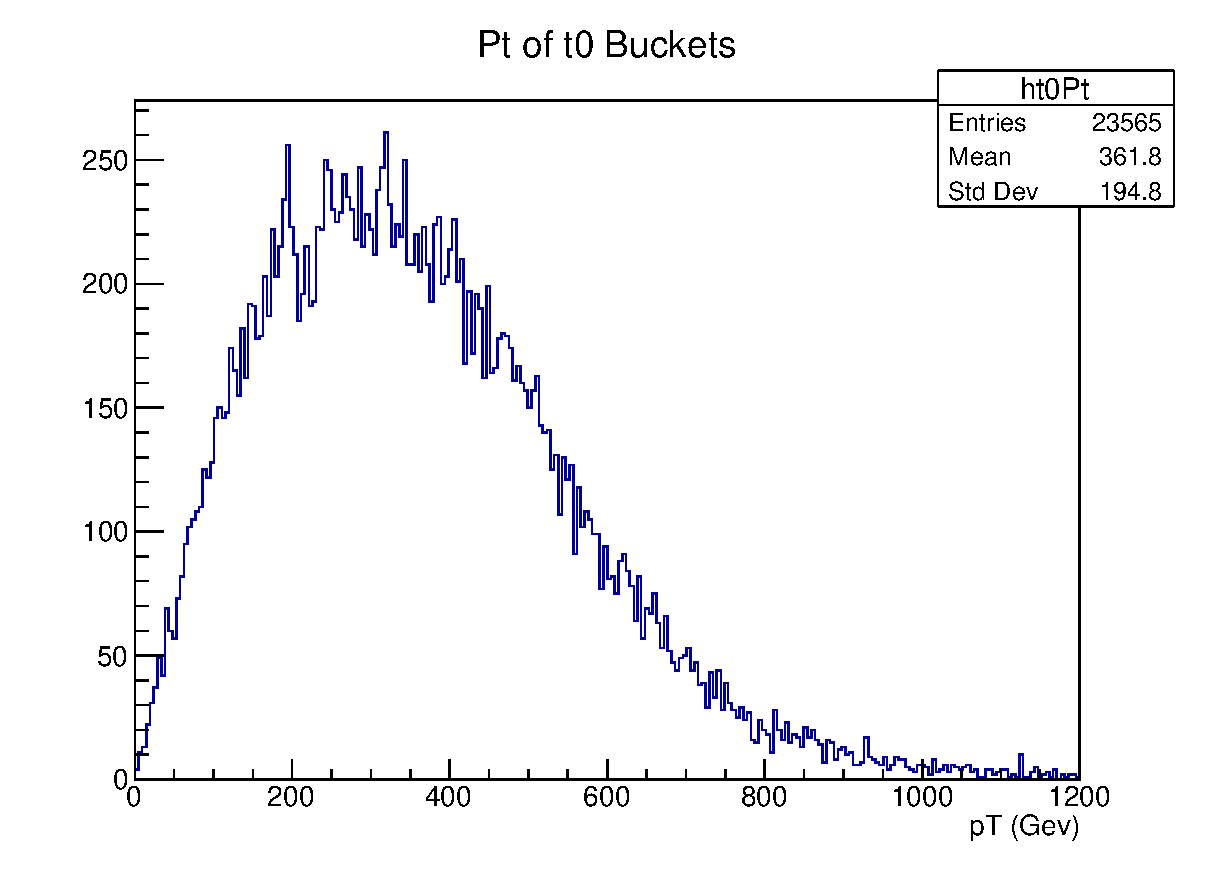
\includegraphics[width=5cm]{ht0Pt_alljetregion.eps}
  \caption{TTHbb}
  \end{subfigure}
  \end{figure}
\end{frame}

\begin{frame}
  \begin{figure}[!h]
  \captionsetup[subfigure]{labelformat=empty}
  \begin{subfigure}{.5\textwidth}
  \centering
  \includegraphics[width=5cm]{reconstructed_top_eta_t0.eps}
  \caption{Chongbin(python)}
  \end{subfigure} \hfill
  \begin{subfigure}{.5\textwidth}
  \centering
  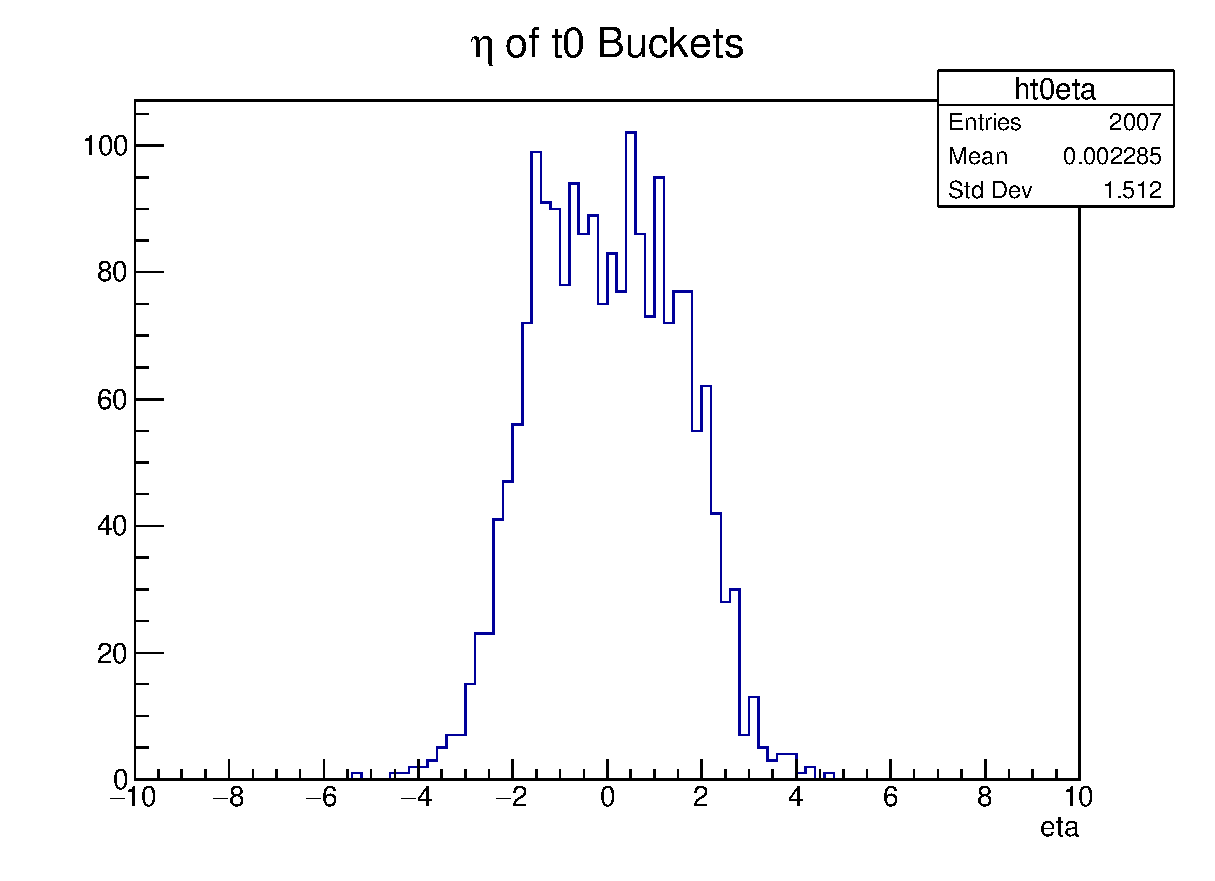
\includegraphics[width=5cm]{ht0eta_alljetregion.eps}
  \caption{TTHbb}
  \end{subfigure}
  \end{figure}
\end{frame}

\begin{frame}
  \begin{figure}[!h]
  \captionsetup[subfigure]{labelformat=empty}
  \begin{subfigure}{.5\textwidth}
  \centering
  \includegraphics[width=5cm]{reconstructed_top_mass_x.eps}
  \caption{Chongbin(python)}
  \end{subfigure} \hfill
  \begin{subfigure}{.5\textwidth}
  \centering
  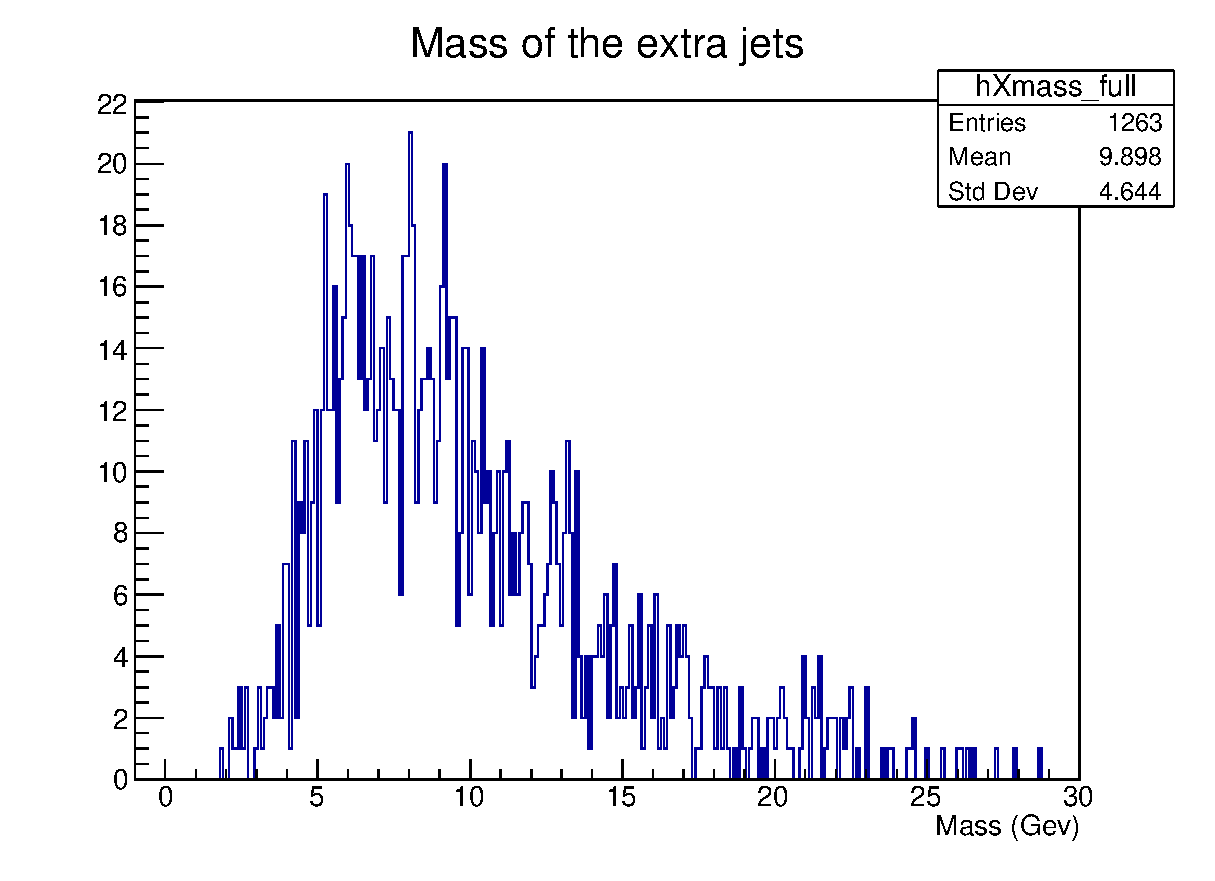
\includegraphics[width=5cm]{hXmass_full_alljetregion.eps}
  \caption{TTHbb}
  \end{subfigure}
  \end{figure}
\end{frame}

\begin{frame}
  \begin{figure}[!h]
  \captionsetup[subfigure]{labelformat=empty}
  \begin{subfigure}{.5\textwidth}
  \centering
  \includegraphics[width=5cm]{reconstructed_top_pt_x.eps}
  \caption{Chongbin(python)}
  \end{subfigure} \hfill
  \begin{subfigure}{.5\textwidth}
  \centering
  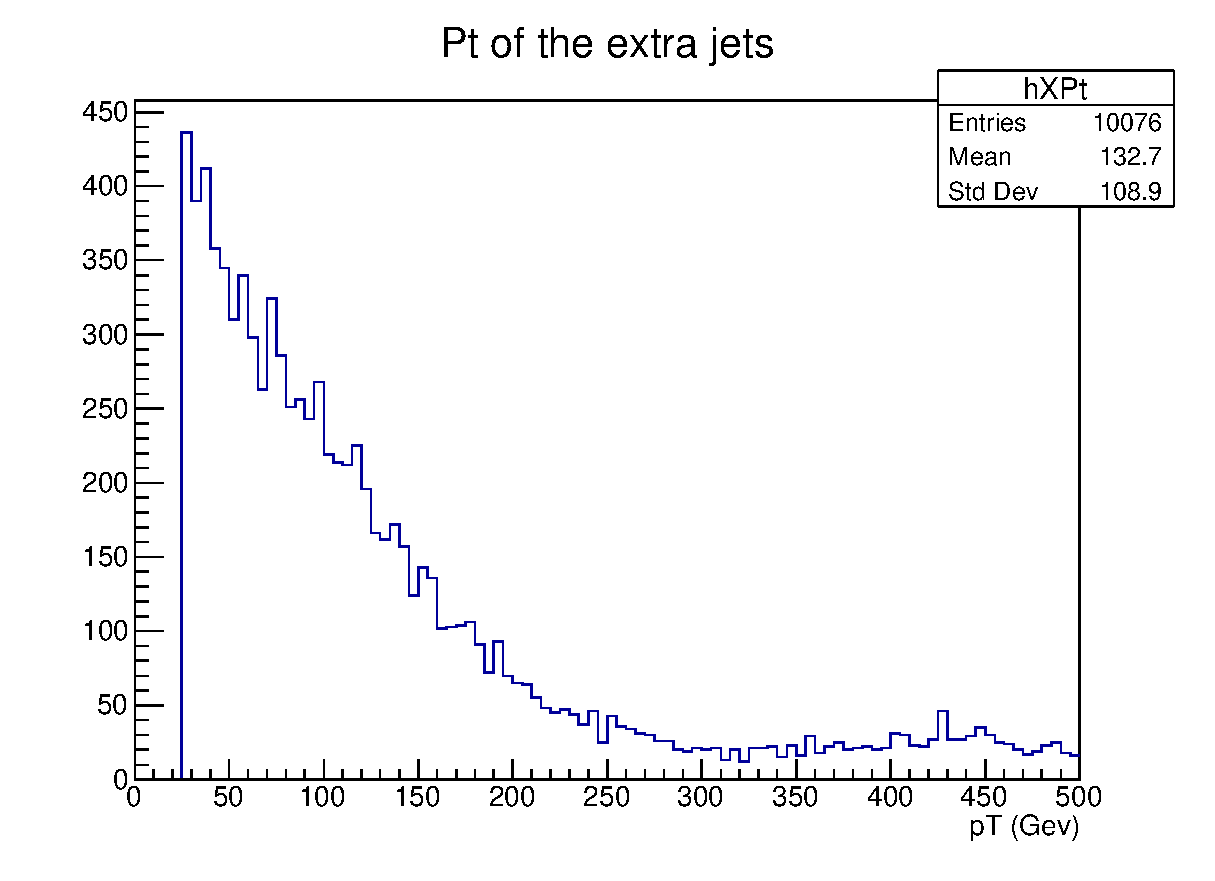
\includegraphics[width=5cm]{hXPt_alljetregion.eps}
  \caption{TTHbb}
  \end{subfigure}
  \end{figure}
\end{frame}

\begin{frame}
  \begin{figure}[!h]
  \captionsetup[subfigure]{labelformat=empty}
  \begin{subfigure}{.5\textwidth}
  \centering
  \includegraphics[width=5cm]{reconstructed_top_eta_x.eps}
  \caption{Chongbin(python)}
  \end{subfigure} \hfill
  \begin{subfigure}{.5\textwidth}
  \centering
  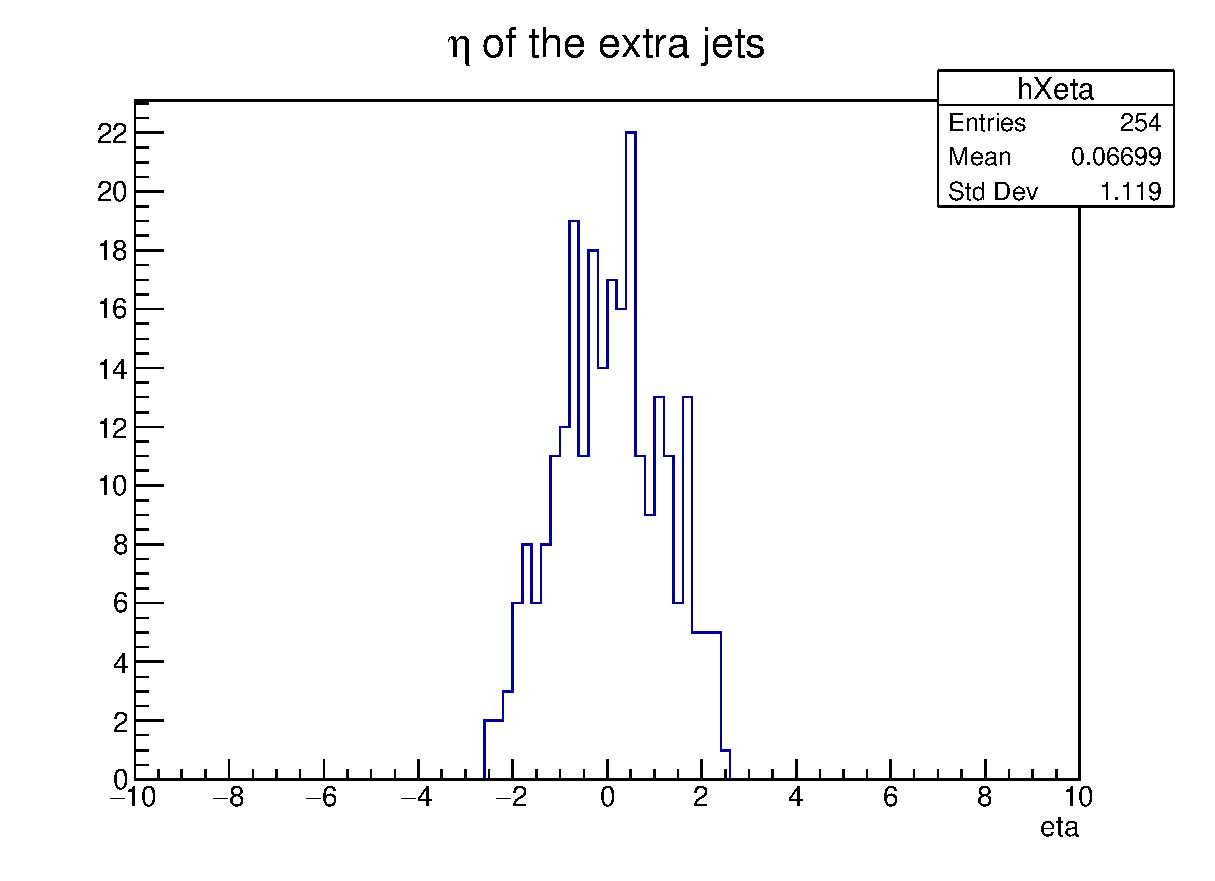
\includegraphics[width=5cm]{hXeta_alljetregion.eps}
  \caption{TTHbb}
  \end{subfigure}
  \end{figure}
\end{frame}

\begin{frame}
  \begin{figure}[!h]
  \captionsetup[subfigure]{labelformat=empty}
  \begin{subfigure}{.5\textwidth}
  \centering
  \includegraphics[width=5cm]{reconstructed_top_m_jk.eps}
  \caption{Chongbin(python)}
  \end{subfigure} \hfill
  \begin{subfigure}{.5\textwidth}
  \centering
  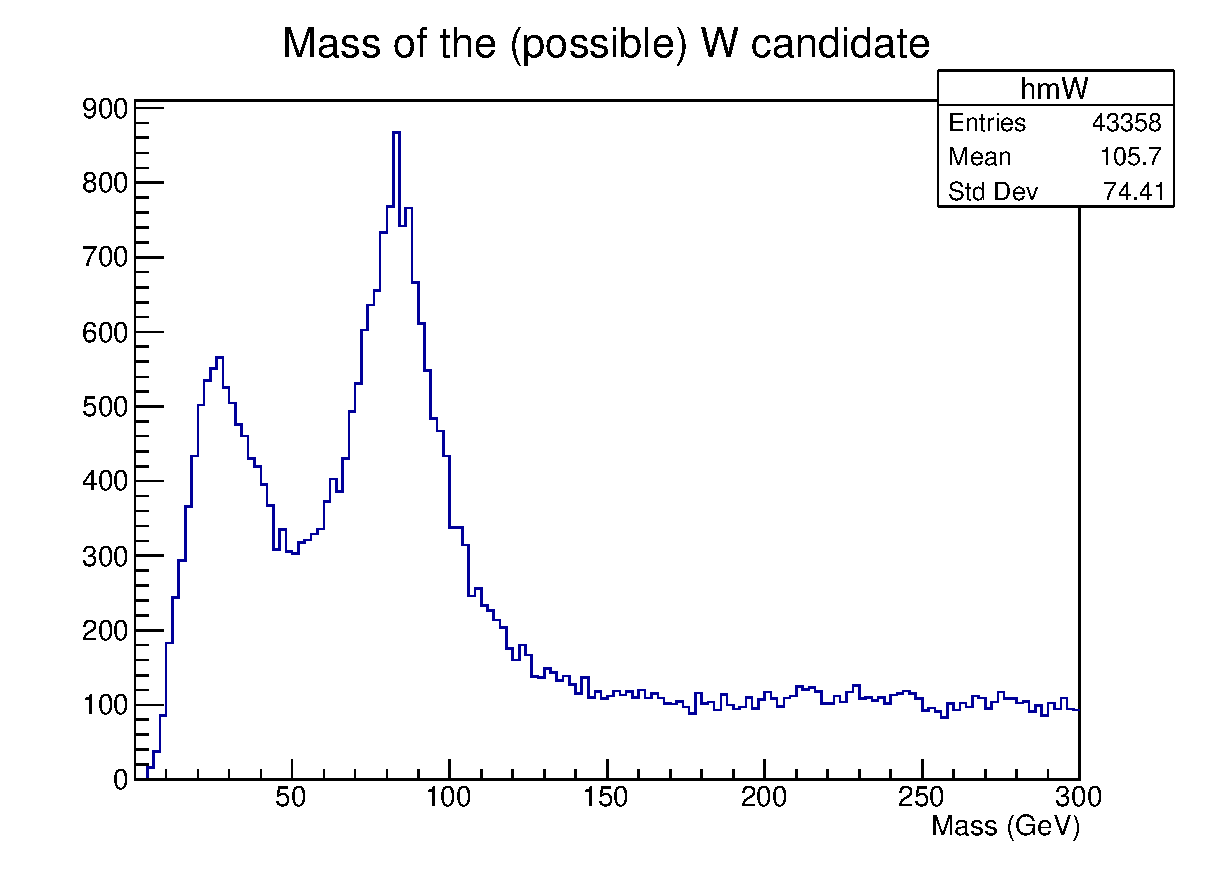
\includegraphics[width=5cm]{hmW_alljetregion.eps}
  \caption{TTHbb}
  \end{subfigure}
  \end{figure}
\end{frame}

\begin{frame}
  \begin{figure}[!h]
  \captionsetup[subfigure]{labelformat=empty}
  \begin{subfigure}{.5\textwidth}
  \centering
  \includegraphics[width=5cm]{reconstructed_top_m_b.eps}
  \caption{Chongbin(python)}
  \end{subfigure} \hfill
  \begin{subfigure}{.5\textwidth}
  \centering
  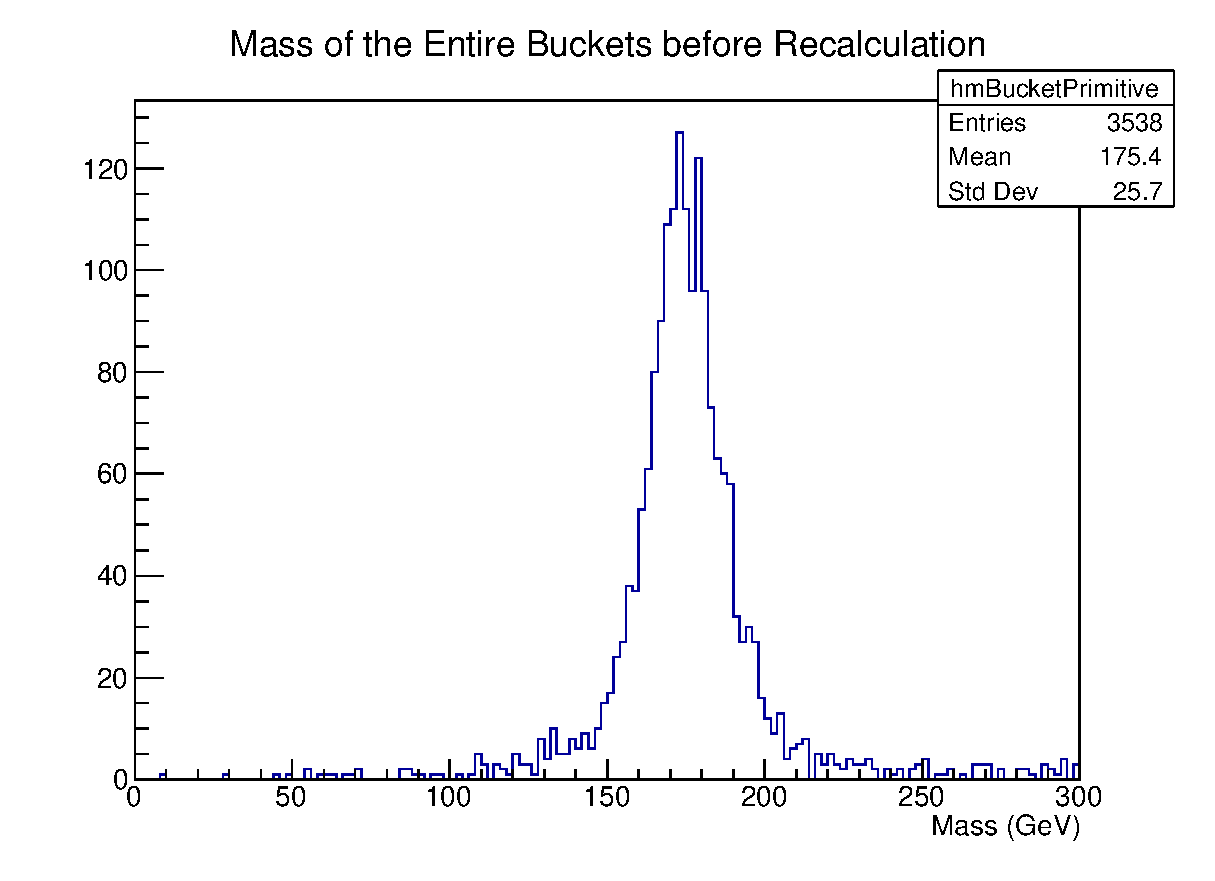
\includegraphics[width=5cm]{hmBucketPrim_alljetregion.eps}
  \caption{TTHbb}
  \end{subfigure}
  \end{figure}
\end{frame}

\begin{frame}
  \begin{figure}[!h]
  \captionsetup[subfigure]{labelformat=empty}
  \begin{subfigure}{.5\textwidth}
  \centering
  \includegraphics[width=5cm]{reconstructed_top_ratio.eps}
  \caption{Chongbin(python)}
  \end{subfigure} \hfill
  \begin{subfigure}{.5\textwidth}
  \centering
  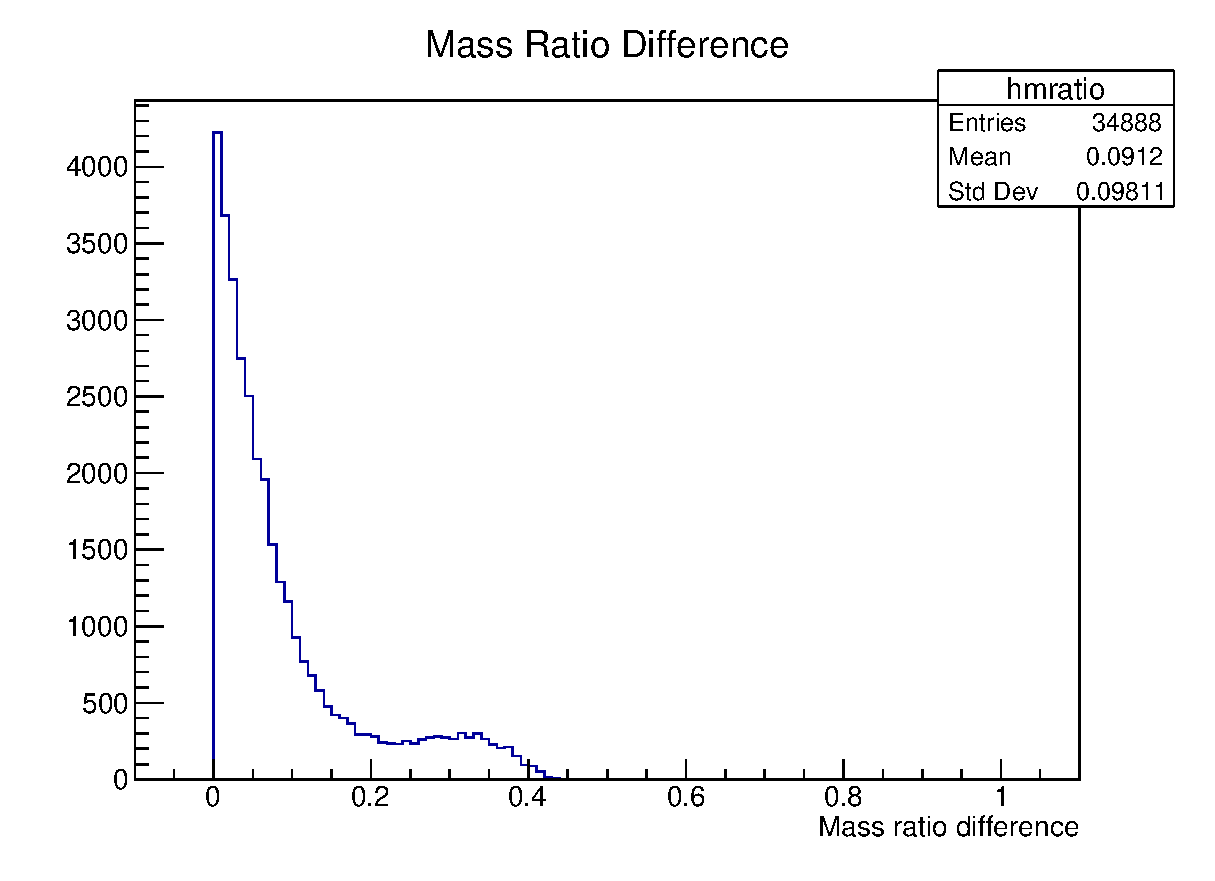
\includegraphics[width=5cm]{hmratio_alljetregion.eps}
  \caption{TTHbb}
  \end{subfigure}
  \end{figure}
\end{frame}

\end{document}
